% ============================================================
%  Chương 2: Thu thập kiến thức về quy định đào tạo
% ============================================================
\chapter{Thu thập kiến thức về quy định đào tạo}
\label{chap:chapter2}

Chương này trình bày tổng quan về hệ thống quy chế đào tạo thạc sĩ tại UIT và ĐHQG-HCM, quy trình thu thập và tổ chức kiến thức từ các văn bản quy phạm, cũng như việc xây dựng bộ câu hỏi kiểm thử phục vụ đánh giá hệ thống. Nội dung chương này tuân theo phương pháp thu thập kiến thức theo miền (domain knowledge acquisition) cho hệ thống truy xuất thông tin.

% ============================================================
\section{Giới thiệu về hệ thống quy chế đào tạo thạc sĩ}
\label{sec:gioithieu_quyche}

% ------------------------------------------------------------
\subsection{Tổng quan hệ thống quy chế đào tạo sau đại học tại Việt Nam}
\label{subsec:tongquan_hethong}

Hệ thống giáo dục sau đại học tại Việt Nam được quản lý bởi nhiều tầng văn bản quy phạm pháp luật, từ cấp quốc gia đến cấp trường. Tại cấp quốc gia, Luật Giáo dục và Luật Giáo dục Đại học đặt ra khung pháp lý chung. Bộ Giáo dục và Đào tạo ban hành các quy chế đào tạo trình độ thạc sĩ, tiến sĩ áp dụng trên toàn quốc. Tại cấp cơ sở, các đại học quốc gia và trường đại học ban hành quy chế riêng phù hợp với đặc thù đào tạo.

Đối với UIT, một trường thành viên của ĐHQG-HCM, hệ thống quy chế đào tạo thạc sĩ bao gồm hai tầng chính:
\begin{itemize}
    \item \textbf{Tầng ĐHQG-HCM}: Các quy chế khung do ĐHQG-HCM ban hành, áp dụng cho tất cả các trường thành viên (QĐ~160, QĐ~1393, QĐ~218).
    \item \textbf{Tầng trường}: Các quy chế, quy định cụ thể hóa do UIT ban hành (QĐ~270, QĐ~851), bổ sung và chi tiết hóa các quy định của ĐHQG-HCM.
\end{itemize}

% ------------------------------------------------------------
\subsection{Cấu trúc văn bản quy phạm}
\label{subsec:cautruc_vanban}

Các văn bản quy chế đào tạo tuân theo cấu trúc phân cấp chuẩn của văn bản quy phạm pháp luật Việt Nam. Từ cấp cao nhất đến cấp thấp nhất, cấu trúc được tổ chức như sau:

\[
\text{Văn bản} \rightarrow \text{Chương} \rightarrow \text{Mục} \rightarrow \text{Điều} \rightarrow \text{Khoản} \rightarrow \text{Điểm}
\]

Mỗi cấp trong hệ thống phân cấp mang một phạm vi quy định riêng biệt. \textit{Văn bản} là đơn vị pháp lý cao nhất, xác định phạm vi và đối tượng áp dụng. \textit{Chương} nhóm các quy định theo chủ đề lớn. \textit{Mục} (nếu có) phân nhỏ chương theo nhóm điều liên quan. \textit{Điều} là đơn vị quy định cơ bản, mang nội dung pháp lý cụ thể. \textit{Khoản} cụ thể hóa từng khía cạnh của Điều. \textit{Điểm} liệt kê các trường hợp hoặc điều kiện chi tiết trong Khoản.

Ngoài cấu trúc phân cấp dọc, các văn bản còn tồn tại các tham chiếu chéo ngang giữa các điều khoản trong cùng một văn bản hoặc giữa các văn bản khác nhau. Ví dụ, để xác định điều kiện bảo vệ luận văn thạc sĩ, cần đọc Điều~24 trong QĐ~270 kết hợp với Điều~25 trong QĐ~1393, hai văn bản thuộc hai tầng quản lý khác nhau.

Hình~\ref{fig:document_tree} minh họa cấu trúc Document Tree của QĐ~270/QĐ-ĐHCNTT với sáu cấp phân cấp và các liên kết tham chiếu chéo giữa các điều.

\begin{figure}[htbp]
    \centering
    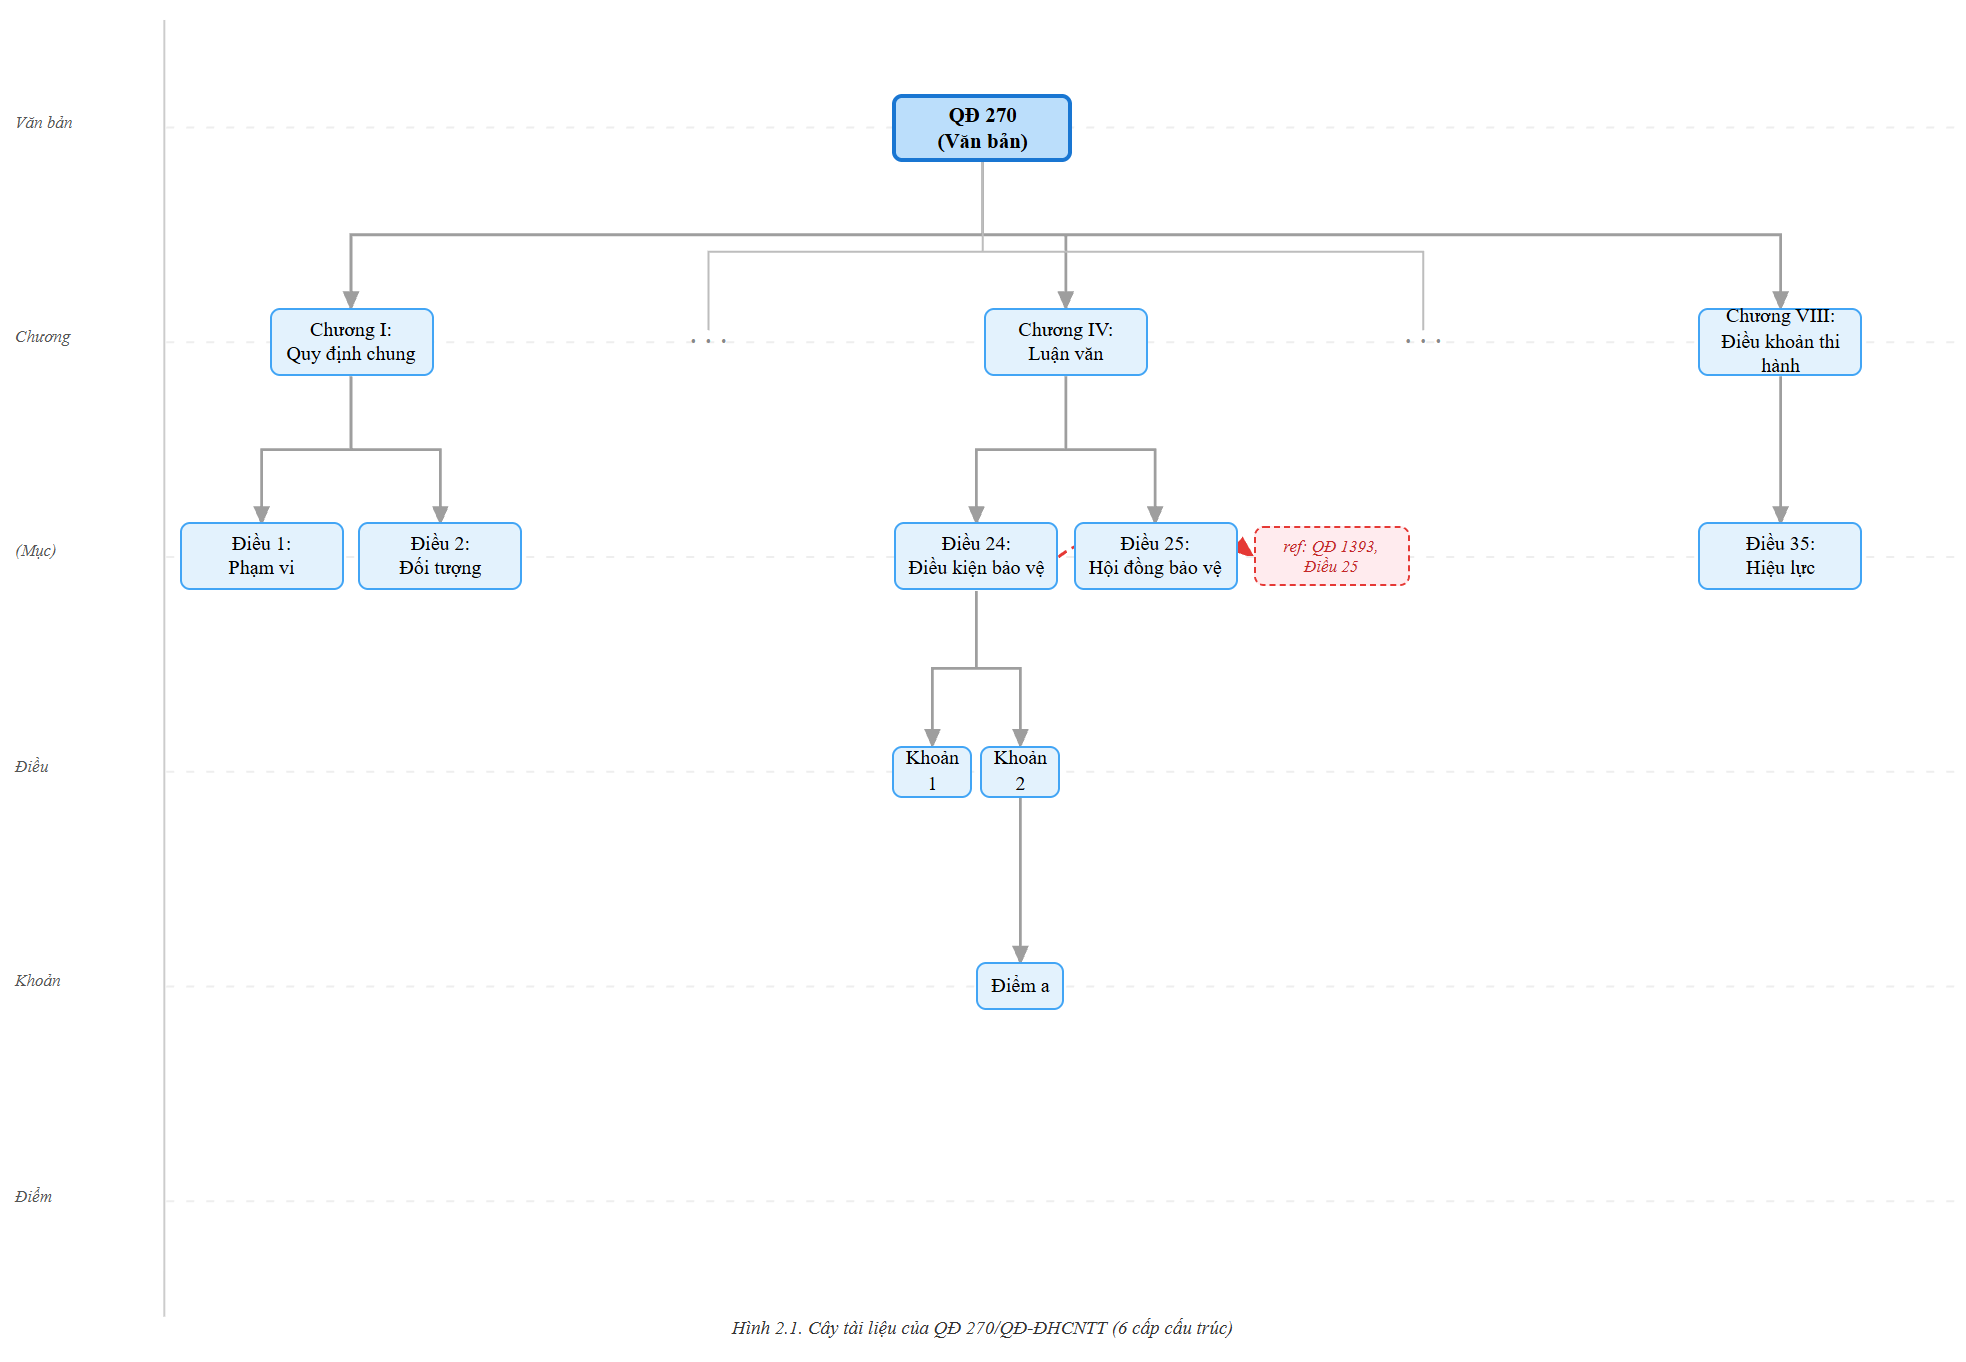
\includegraphics[width=0.95\textwidth]{graphics/figure2-1-document-tree.png}
    \caption{Cấu trúc Document Tree của QĐ~270/QĐ-ĐHCNTT (minh họa rút gọn). Mũi tên nét đứt thể hiện tham chiếu chéo giữa các điều.}
    \label{fig:document_tree}
\end{figure}

% ------------------------------------------------------------
\subsection{Các quy chế trong phạm vi nghiên cứu}
\label{subsec:cacquiche}

Bảng~\ref{tab:quyche_list} liệt kê năm văn bản quy chế đào tạo trong phạm vi nghiên cứu của luận văn.

\begin{table}[htbp]
    \centering
    \caption{Danh sách các quy chế đào tạo trong phạm vi nghiên cứu}
    \label{tab:quyche_list}
    \begin{tabular}{clccc}
        \toprule
        \textbf{STT} & \textbf{Tên quy chế} & \textbf{Số QĐ} & \textbf{Số chương} & \textbf{Số điều} \\
        \midrule
        1 & Quy chế ĐT trình độ ThS của UIT
          & 270/QĐ-ĐHCNTT & 8 & 35 \\
        2 & Quy chế ĐT trình độ ThS ĐHQG-HCM (khóa 2021)
          & 160/QĐ-ĐHQG & 7 & 28 \\
        3 & Quy chế ĐT trình độ ThS ĐHQG-HCM (khóa 2022+)
          & 1393/QĐ-ĐHQG & 8 & 32 \\
        4 & Quy chế sửa đổi bổ sung về GVHD
          & 218/QĐ-ĐHQG & 2 & 6 \\
        5 & Quy định liêm chính học thuật
          & 851/QĐ-ĐHCNTT & 3 & 8 \\
        \midrule
        \multicolumn{3}{r}{\textbf{Tổng cộng}} & \textbf{28} & \textbf{109} \\
        \bottomrule
    \end{tabular}
\end{table}

\textbf{QĐ~270/QĐ-ĐHCNTT} là quy chế đào tạo thạc sĩ chủ đạo của UIT, ban hành ngày 25/04/2022. Quy chế gồm 8~chương và 35~điều, bao phủ toàn bộ quy trình đào tạo thạc sĩ tại UIT từ tuyển sinh, tổ chức đào tạo, đến bảo vệ và cấp bằng. Đây là văn bản cụ thể hóa các quy định của ĐHQG-HCM, có tính đặc thù cao cho UIT.

\textbf{QĐ~160/QĐ-ĐHQG} là quy chế đào tạo thạc sĩ của ĐHQG-HCM áp dụng cho khóa tuyển sinh năm 2021 trở về trước, gồm 7~chương và 28~điều, quy định về tổ chức và quản lý đào tạo trình độ thạc sĩ trong toàn hệ thống ĐHQG-HCM.

\textbf{QĐ~1393/QĐ-ĐHQG} là quy chế thay thế QĐ~160 áp dụng từ khóa tuyển sinh năm 2022 trở đi, gồm 8~chương và 32~điều. Quy chế này có nhiều điểm mới về yêu cầu ngoại ngữ, điều kiện bảo vệ luận văn và hình thức đào tạo.

\textbf{QĐ~218/QĐ-ĐHQG} là quy chế sửa đổi bổ sung một số điều liên quan đến giảng viên hướng dẫn (GVHD), gồm 2~chương và 6~điều. Quy chế này bổ sung và cập nhật các tiêu chuẩn, trách nhiệm của GVHD luận văn thạc sĩ.

\textbf{QĐ~851/QĐ-ĐHCNTT} quy định về liêm chính học thuật tại UIT, gồm 3~chương và 8~điều, nêu rõ các hành vi vi phạm liêm chính học thuật và chế tài xử lý đối với học viên cao học.

% ============================================================
\section{Thu thập kiến thức trong văn bản quy chế}
\label{sec:thuthap_kienthuc}

% ------------------------------------------------------------
\subsection{Quy trình thu thập và số hóa}
\label{subsec:quytrinh_thuthap}

Quy trình thu thập và số hóa kiến thức từ các văn bản quy phạm được thực hiện qua bốn bước tuần tự:

\begin{enumerate}
    \item \textbf{Thu thập văn bản gốc}: Các quy chế, quy định được thu thập từ cổng thông tin điện tử của UIT và ĐHQG-HCM dưới định dạng PDF và Word. Văn bản được kiểm tra tính xác thực và cập nhật nhất trước khi đưa vào xử lý.

    \item \textbf{Phân tích cấu trúc}: Mỗi văn bản được phân tích thủ công để xác định cấu trúc phân cấp (Chương, Mục, Điều, Khoản, Điểm). Dữ liệu cấu trúc được mã hóa thành JSON theo schema chuẩn, tạo thành Document Tree cho từng văn bản.

    \item \textbf{Trích xuất tham chiếu chéo}: Các tham chiếu chéo giữa các điều, khoản trong cùng một văn bản hoặc giữa các văn bản được xác định và ghi nhận dưới dạng cạnh trong Knowledge Graph. Việc trích xuất kết hợp quy tắc regex và kiểm tra thủ công để đảm bảo độ chính xác.

    \item \textbf{Tạo tóm tắt}: Mỗi Điều và mỗi Chương được tóm tắt tự động bằng mô hình Claude~3.5~Haiku (Anthropic). Tóm tắt phục vụ cho việc nhúng vector và tra cứu ngữ nghĩa ở Tầng~2 của hệ thống truy xuất.
\end{enumerate}

% ------------------------------------------------------------
\subsection{Các khái niệm chính}
\label{subsec:khainiemchinh}

Quá trình phân tích các văn bản quy chế xác định bảy loại khái niệm chính được biểu diễn trong Knowledge Graph:

\begin{enumerate}
    \item \textbf{Hành động} (Action): Các hoạt động trong quy trình đào tạo, ví dụ: \textit{đăng ký học phần}, \textit{bảo vệ luận văn}, \textit{xét tốt nghiệp}.
    \item \textbf{Điều kiện} (Condition): Các yêu cầu phải thỏa mãn để thực hiện một hành động, ví dụ: \textit{hoàn thành tín chỉ}, \textit{đạt chuẩn ngoại ngữ}.
    \item \textbf{Tổ chức} (Organization): Các đơn vị liên quan, ví dụ: \textit{Phòng Đào tạo Sau Đại học}, \textit{Hội đồng bảo vệ luận văn}.
    \item \textbf{Người} (Person): Các vai trò chủ thể, ví dụ: \textit{học viên cao học}, \textit{giảng viên hướng dẫn}, \textit{phản biện}.
    \item \textbf{Tham chiếu pháp lý} (Legal Reference): Các điều, khoản được trích dẫn chéo, ví dụ: \textit{Điều 24 QĐ 270}, \textit{Khoản 2 Điều 15 QĐ 1393}.
    \item \textbf{Thời hạn} (Deadline): Các mốc thời gian và ràng buộc, ví dụ: \textit{trong vòng 24 tháng}, \textit{trước ngày 30 tháng 6}.
    \item \textbf{Chế tài} (Sanction): Hậu quả pháp lý khi vi phạm, ví dụ: \textit{buộc thôi học}, \textit{hủy kết quả bảo vệ}.
\end{enumerate}

% ------------------------------------------------------------
\subsection{Các quan hệ giữa các khái niệm}
\label{subsec:quanhe}

Knowledge Graph biểu diễn năm loại quan hệ chính giữa các khái niệm:

\begin{enumerate}
    \item \textbf{requires} (yêu cầu): Liên kết Hành động với Điều kiện tiên quyết. Ví dụ: \textit{bảo vệ luận văn} \texttt{requires} \textit{hoàn thành tín chỉ}.
    \item \textbf{leads\_to} (dẫn đến): Liên kết Hành động với kết quả hoặc Hành động tiếp theo. Ví dụ: \textit{bảo vệ luận văn đạt} \texttt{leads\_to} \textit{xét tốt nghiệp}.
    \item \textbf{regulates} (quy định): Liên kết Tham chiếu pháp lý với Hành động hoặc Điều kiện được điều chỉnh. Ví dụ: \textit{Điều 24 QĐ 270} \texttt{regulates} \textit{điều kiện bảo vệ luận văn}.
    \item \textbf{references} (tham chiếu): Liên kết giữa các Tham chiếu pháp lý có nội dung liên quan, thể hiện tham chiếu chéo. Ví dụ: \textit{Điều 24 QĐ 270} \texttt{references} \textit{Điều 25 QĐ 1393}.
    \item \textbf{involves} (liên quan): Liên kết Hành động hoặc Điều kiện với Tổ chức hoặc Người có thẩm quyền. Ví dụ: \textit{bảo vệ luận văn} \texttt{involves} \textit{Hội đồng bảo vệ}.
\end{enumerate}

Hình~\ref{fig:kg_subgraph} minh họa một đồ thị con của Knowledge Graph xoay quanh khái niệm \textit{``bảo vệ luận văn thạc sĩ''}, thể hiện các loại nút và cạnh quan hệ khác nhau.

\begin{figure}[htbp]
    \centering
    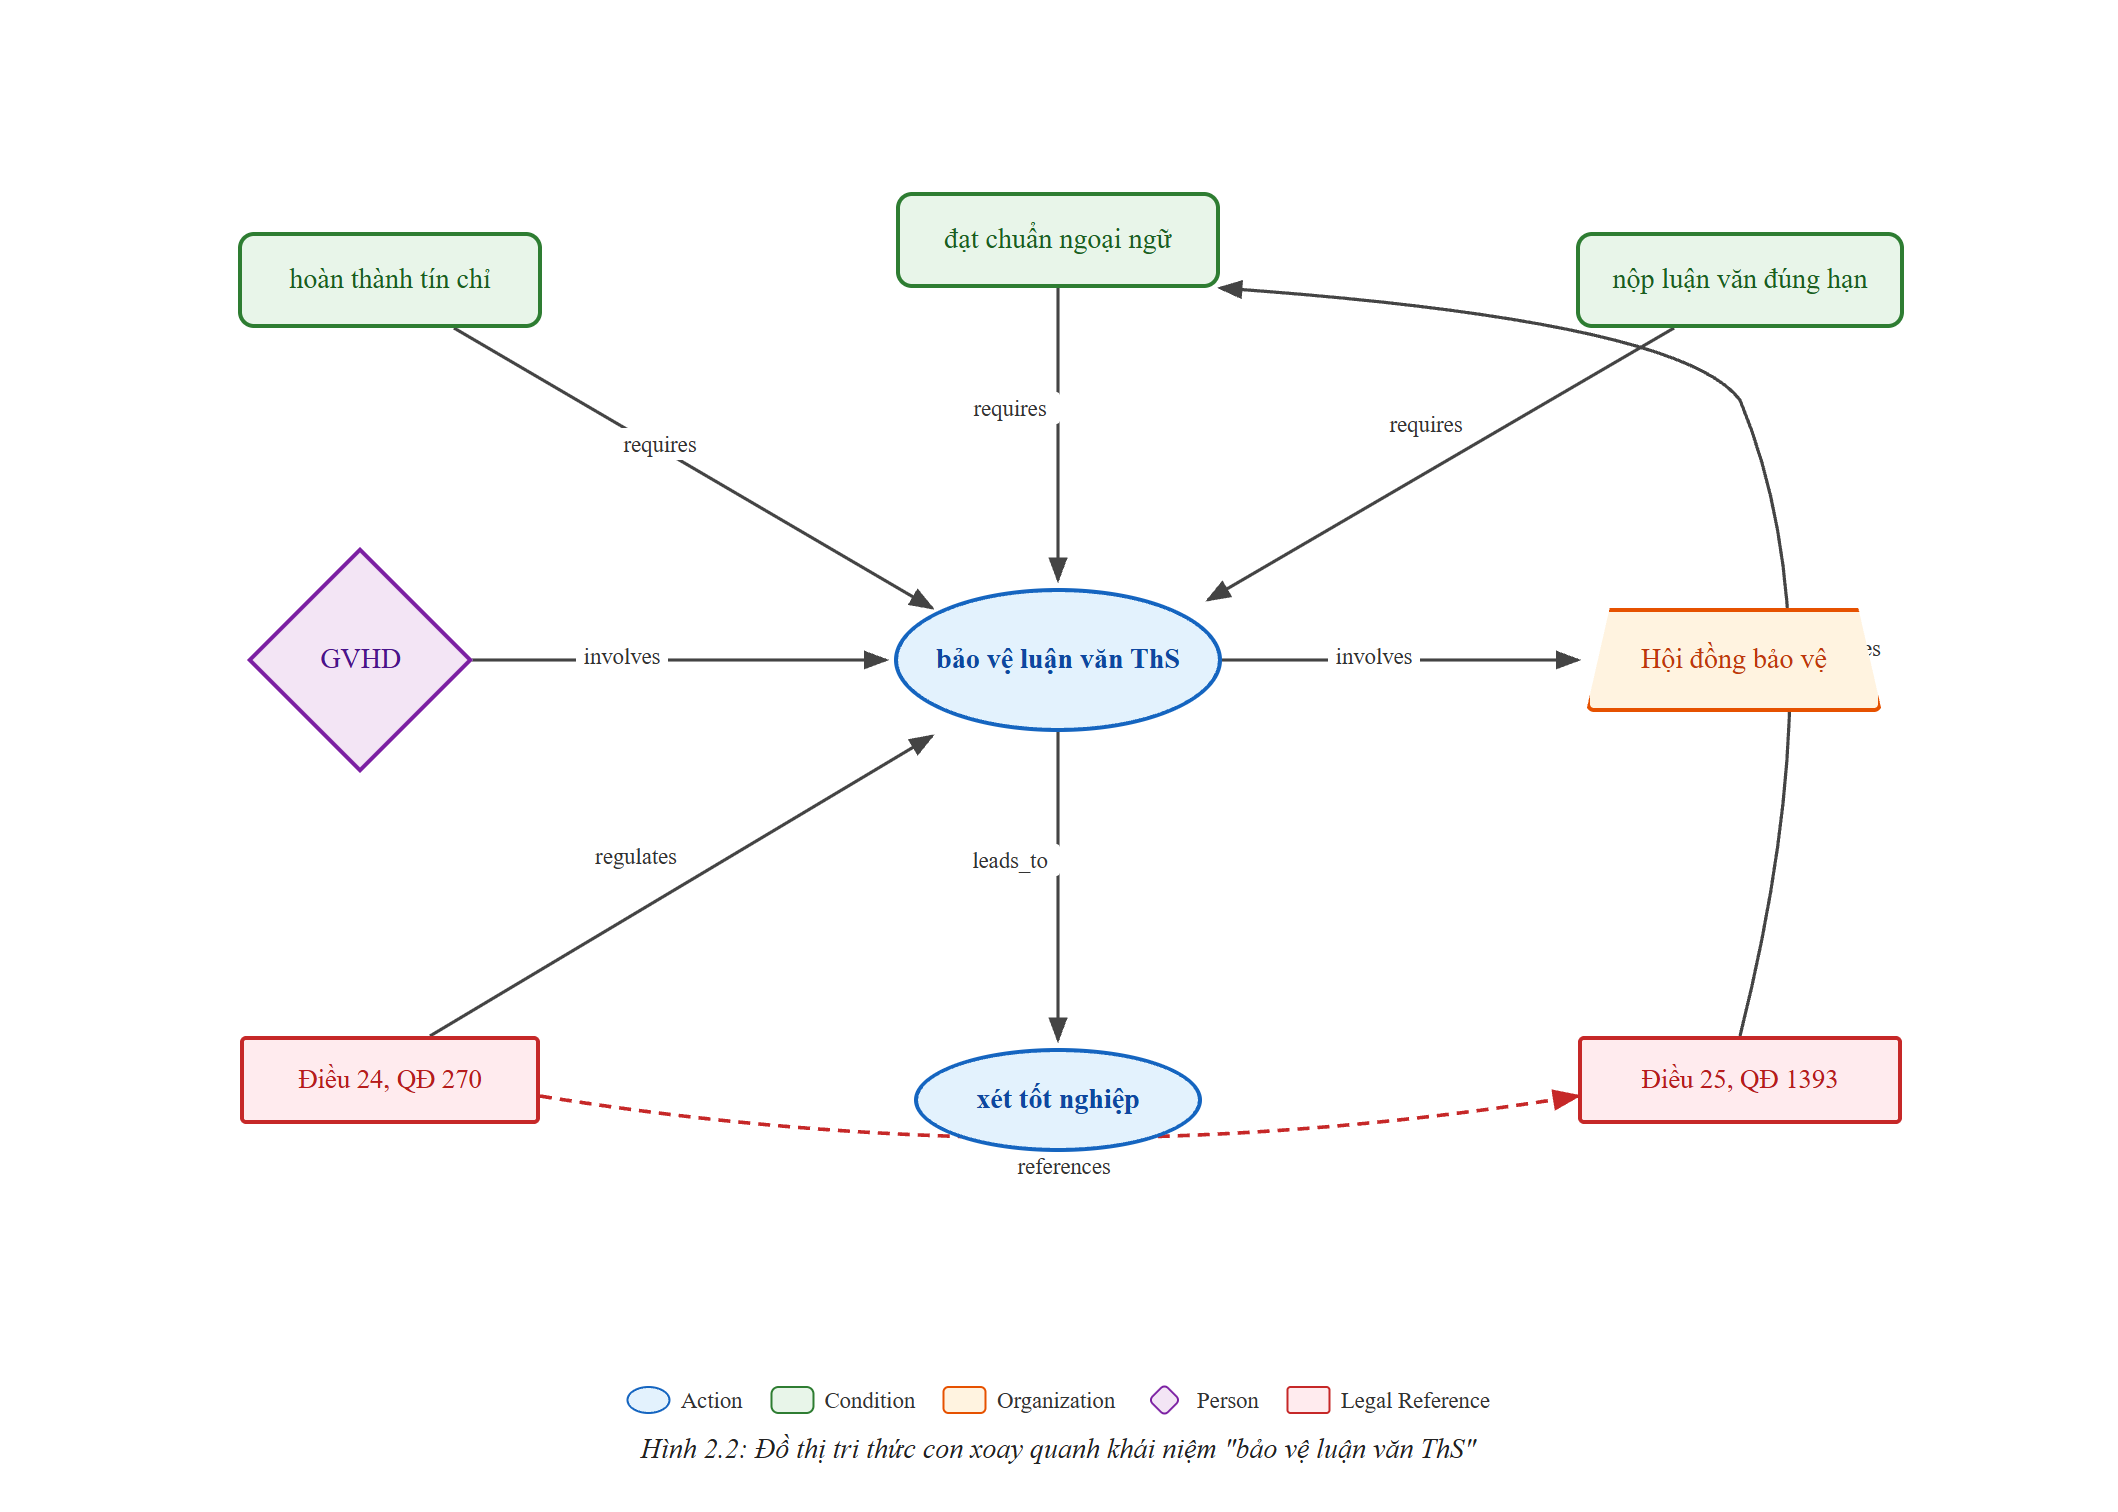
\includegraphics[width=0.95\textwidth]{graphics/figure2-2-kg-subgraph.png}
    \caption{Đồ thị con minh họa Knowledge Graph xoay quanh khái niệm \textit{``bảo vệ luận văn thạc sĩ''}. Hình elip xanh: Hành động; Hình chữ nhật bo góc xanh lá: Điều kiện; Hình thang cam: Tổ chức; Hình thoi tím: Người; Hình chữ nhật đỏ: Tham chiếu pháp lý.}
    \label{fig:kg_subgraph}
\end{figure}

% ------------------------------------------------------------
\subsection{Phân loại chủ đề}
\label{subsec:phanloa_chude}

Nội dung các quy chế đào tạo thạc sĩ được phân loại thành bảy chủ đề chính phục vụ cho việc định tuyến ý định và tổ chức Knowledge Graph. Bảng~\ref{tab:chude_phanloa} trình bày chi tiết bảy chủ đề cùng các từ khóa đặc trưng.

\begin{table}[htbp]
    \centering
    \caption{Phân loại chủ đề trong quy chế đào tạo thạc sĩ}
    \label{tab:chude_phanloa}
    \begin{tabular}{clp{7cm}}
        \toprule
        \textbf{STT} & \textbf{Chủ đề} & \textbf{Từ khóa đặc trưng} \\
        \midrule
        1 & Tuyển sinh và nhập học
          & điều kiện dự tuyển, hồ sơ tuyển sinh, nhập học, chỉ tiêu \\
        2 & Tổ chức đào tạo
          & chương trình học, học phần, tín chỉ, kế hoạch học tập \\
        3 & Giảng viên hướng dẫn
          & GVHD, tiêu chuẩn hướng dẫn, phân công, thay đổi GVHD \\
        4 & Luận văn thạc sĩ
          & đề tài, đề cương, viết luận văn, nộp luận văn \\
        5 & Bảo vệ và tốt nghiệp
          & hội đồng bảo vệ, điều kiện bảo vệ, xét tốt nghiệp, cấp bằng \\
        6 & Ngoại ngữ và liêm chính
          & chuẩn ngoại ngữ, chứng chỉ, đạo văn, liêm chính học thuật \\
        7 & Kỷ luật và khiếu nại
          & vi phạm, xử lý kỷ luật, thôi học, khiếu nại, phúc khảo \\
        \bottomrule
    \end{tabular}
\end{table}

% ============================================================
\section{Thu thập câu hỏi kiểm thử}
\label{sec:cau_hoi_kiem_thu}

% ------------------------------------------------------------
\subsection{Nguồn thu thập}
\label{subsec:nguon_thuthap}

Bộ câu hỏi kiểm thử được xây dựng từ hai nguồn chính:

\textbf{Miền quy định đào tạo} (130 câu hỏi): Câu hỏi được thu thập từ các diễn đàn trực tuyến, nhóm Facebook của học viên cao học UIT và ĐHQG-HCM, các buổi tư vấn tuyển sinh được ghi âm, và các thắc mắc học viên gửi đến Phòng Đào tạo Sau Đại học. Câu hỏi phản ánh nhu cầu tra cứu thực tế của học viên, từ các vấn đề cơ bản đến các tình huống phức tạp đòi hỏi kết nối nhiều điều khoản từ nhiều văn bản.

\textbf{Miền pháp luật Việt Nam} (400 câu hỏi): Câu hỏi được thu thập từ nhóm Facebook về tư vấn pháp luật, bao gồm các vấn đề thuộc lĩnh vực luật doanh nghiệp và luật giao thông đường bộ. Tập dữ liệu này phục vụ đánh giá tính tổng quát của hệ thống trên miền pháp lý mở rộng (Chương~\ref{chap:chapter4}).

% ------------------------------------------------------------
\subsection{Phân loại câu hỏi}
\label{subsec:phanloa_cauhoi}

Câu hỏi được phân loại theo độ phức tạp suy luận thành ba loại:

\begin{itemize}
    \item \textbf{Single-hop}: Câu hỏi có thể trả lời từ một điều khoản duy nhất trong một văn bản. Ví dụ: \textit{``Học viên cần bao nhiêu tín chỉ để hoàn thành chương trình thạc sĩ tại UIT?''}

    \item \textbf{Multi-hop}: Câu hỏi đòi hỏi kết nối thông tin từ nhiều điều khoản trong cùng một hoặc nhiều văn bản khác nhau. Ví dụ: \textit{``Học viên cao học nhập học năm 2022 cần đáp ứng những điều kiện gì để được bảo vệ luận văn?''} (cần kết hợp QĐ~270 và QĐ~1393).

    \item \textbf{Reasoning}: Câu hỏi đòi hỏi suy luận logic trên nhiều điều kiện, so sánh các tình huống hoặc xác định hành vi hợp lệ/vi phạm. Ví dụ: \textit{``Nếu học viên đã hết thời hạn đào tạo nhưng chưa bảo vệ luận văn, những phương án nào có thể thực hiện?''}
\end{itemize}

% ------------------------------------------------------------
\subsection{Thống kê bộ câu hỏi}
\label{subsec:thongke_cauhoi}

Bảng~\ref{tab:thongke_cauhoi} trình bày thống kê bộ câu hỏi kiểm thử miền quy định đào tạo thạc sĩ theo chủ đề và loại câu hỏi.

\begin{table}[htbp]
    \centering
    \caption{Thống kê bộ câu hỏi kiểm thử miền quy định đào tạo (tổng 130 câu)}
    \label{tab:thongke_cauhoi}
    \begin{tabular}{clccc r}
        \toprule
        \textbf{STT} & \textbf{Chủ đề}
            & \textbf{Single-hop} & \textbf{Multi-hop} & \textbf{Reasoning}
            & \textbf{Tổng (\%)} \\
        \midrule
        1 & Tuyển sinh và nhập học     & 10 &  5 &  3 & 18\,(13,8\%) \\
        2 & Tổ chức đào tạo            & 12 &  7 &  4 & 23\,(17,7\%) \\
        3 & Giảng viên hướng dẫn       &  6 &  5 &  3 & 14\,(10,8\%) \\
        4 & Luận văn thạc sĩ           &  8 &  8 &  4 & 20\,(15,4\%) \\
        5 & Bảo vệ và tốt nghiệp       &  7 & 10 &  5 & 22\,(16,9\%) \\
        6 & Ngoại ngữ và liêm chính    &  6 &  5 &  3 & 14\,(10,8\%) \\
        7 & Kỷ luật và khiếu nại       &  5 &  7 &  7 & 19\,(14,6\%) \\
        \midrule
        \multicolumn{2}{l}{\textbf{Tổng cộng}}
            & \textbf{54} & \textbf{47} & \textbf{29}
            & \textbf{130\,(100\%)} \\
        \bottomrule
    \end{tabular}
\end{table}

Bảng~\ref{tab:vidu_cauhoi} cung cấp mười câu hỏi mẫu đại diện từ bộ kiểm thử, kèm theo các điều khoản vàng (gold articles) được xác định thủ công bởi chuyên gia.

\begin{table}[htbp]
    \centering
    \caption{Ví dụ câu hỏi mẫu từ bộ kiểm thử}
    \label{tab:vidu_cauhoi}
    \begin{tabular}{p{0.4cm} p{6.2cm} p{2.0cm} p{3.6cm}}
        \toprule
        \textbf{STT} & \textbf{Câu hỏi} & \textbf{Loại} & \textbf{Gold articles} \\
        \midrule
        1 & Học viên cao học tại UIT cần hoàn thành bao nhiêu tín chỉ?
          & Single-hop & Điều 5, QĐ 270 \\
        2 & Điều kiện để được đăng ký bảo vệ luận văn thạc sĩ là gì?
          & Multi-hop & Điều 24 QĐ 270; Điều 25 QĐ 1393 \\
        3 & Học viên nhập học năm 2022 cần đạt chuẩn ngoại ngữ như thế nào?
          & Single-hop & Điều 25, QĐ 1393 \\
        4 & GVHD luận văn thạc sĩ cần đáp ứng tiêu chuẩn gì theo QĐ 218?
          & Single-hop & Điều 2, QĐ 218 \\
        5 & Hành vi đạo văn bị xử lý như thế nào tại UIT?
          & Single-hop & Điều 6, QĐ 851 \\
        6 & Học viên hết hạn 24 tháng chưa bảo vệ thì có thể xin gia hạn không?
          & Reasoning & Điều 12 QĐ 270; Điều 18 QĐ 1393 \\
        7 & Hội đồng bảo vệ luận văn ThS gồm những thành phần nào?
          & Single-hop & Điều 26, QĐ 270 \\
        8 & Nếu học viên bị đình chỉ học, điều kiện để được học lại là gì?
          & Reasoning & Điều 30 QĐ 270; Điều 22 QĐ 1393 \\
        9 & Học viên có thể thay đổi GVHD trong quá trình làm luận văn không?
          & Multi-hop & Điều 3 QĐ 218; Điều 18 QĐ 270 \\
        10 & Thủ tục nộp luận văn sau bảo vệ để được cấp bằng thạc sĩ?
           & Multi-hop & Điều 28 QĐ 270; Điều 27 QĐ 1393 \\
        \bottomrule
    \end{tabular}
\end{table}
